\section{Motivation}
\label{sec:motivation}

\begin{figure}[t]
\centering
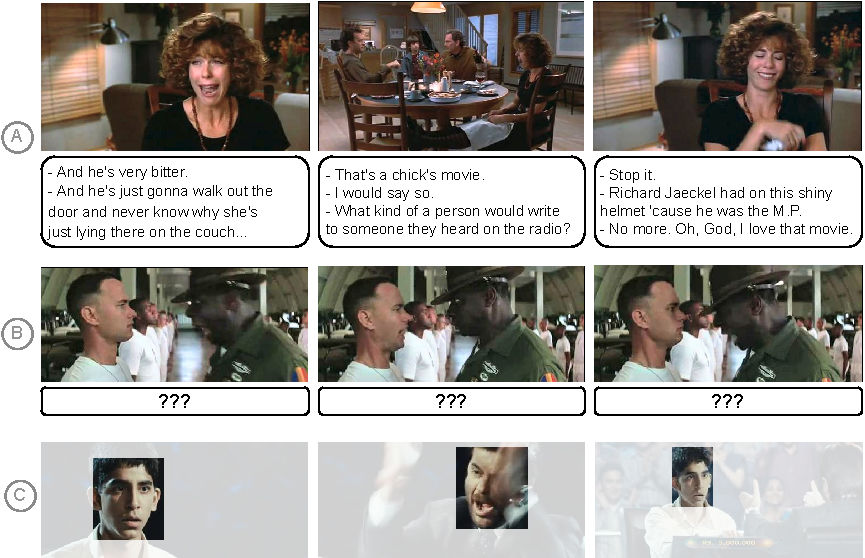
\includegraphics[width=0.7\linewidth]{Figures/teaser.pdf}
\vspace{-4mm}
\caption{Multimodal models and multi-label emotions are necessary for understanding the story.
\textbf{A}: What character emotions can we sense in this scene?
Is a single label enough?
\textbf{B}: Without the dialog, can we try to guess the emotions of the Sergeant and the Soldier.
\textbf{C}: Is it possible to infer the emotions from the characters' facial expressions (without subtitles and visual background) only?
Check the footnote below for the ground-truth emotion labels for these scenes.}
\label{fig:teaser}
\end{figure}

Emotions are a deeply-studied topic.
From ancient Rome and Cicero's 4-way classification~\cite{cicero-emo}, to modern brain research~\cite{progbrainres}, emotions have fascinated humanity.
Psychologists use of Plutchik's wheel~\cite{plutchik} or the proposal of universality in facial expressions by Ekman~\cite{Ekman1971}, structure has been provided to this field through various theories.
Affective emotions are also grouped into mental (affective, behavioral, and cognitive) or bodily states~\cite{clore1987affectivelexicon}.

\blfootnote{%Emotion labels for each clip:
Ground-truth emotions and mental states portrayed in Fig.~\ref{fig:teaser}:
\textbf{A}: excited, curious, confused, annoyed, alarmed;
\textbf{B}: shocked, confident (sergeant praises the soldier with agressive tone);
\textbf{C}: happy, excited, amused, shocked, confident, nervous.}

A recent work on recognizing emotions with visual context, Emotic~\cite{emotic} identifies 26 label clusters and proposes a \emph{multi-label} setup wherein an image may exhibit multiple emotions (\eg~\emph{peace, engagement}).
An alternative to the categorical space, valence, arousal, and dominance are also used as three continuous dimensions~\cite{emotic}.

Predicting a rich set of emotions requires analyzing multiple contextual modalities~\cite{emotic, caer, emoticon}.
Popular directions in multimodal emotion recognition are
Emotion Recognition in Conversations (ERC) that classifies the emotion for every dialog utterance~\cite{poria2019meld, dialogRNN, todkat};
or predicting a single valence-activity score for short $\sim$10s movie clips~\cite{BaveyeLIRIS, affect2mm}.

Classification in a rich label space of emotions requires looking at multimodal context as evident from masking context in Fig.~\ref{fig:teaser}.
To this end, we propose \modelname{} that jointly models video frames, dialog utterances, and character appearance.

\modelname{} operates at the level of a \emph{movie scene}: a set of shots telling a sub-story, typically at one location, among a defined cast, and in a short time span of 30-60s.
Thus, scenes are considerably longer than single dialogs~\cite{poria2019meld} or movie clips in~\cite{BaveyeLIRIS}.
\modelname{} predict emotions and mental states for all characters in the scene and also by accumulating labels at the scene level.
Estimation on a larger time window naturally lends itself to multi-label classification as characters may portray multiple emotions simultaneously (\eg~\emph{curious} and \emph{confused}) or have transitions due to interactions with other characters (\eg~\emph{worried} to \emph{calm}).


\vspace{-3mm}
